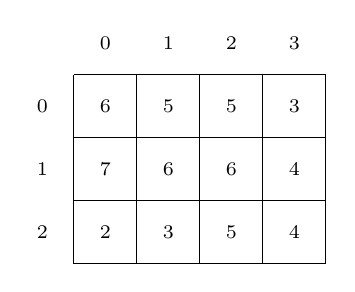
\begin{tikzpicture}[x=0.8cm, y=0.8cm]
%Ranga Rodrigo
%December 1, 2017
\def\rows{3}
\def\cols{4}
\def\printindices{false}
\def\printimagevalues{true}

\begin{filecontents*}{interpimage.dat}
2
3
5
4
7
6
6
4
6
5
5
3
\end{filecontents*}



\foreach \i in {0,1, ..., \rows}
{
	\draw[black] (0, \i)  -- ++(\cols, 0);
}
\foreach \j in {0,1, ..., \cols}
{
	\draw[black] (\j, 0)  -- ++(0, \rows);
}


\pgfmathsetmacro{\rowsminusone}{\rows -1 }%
\pgfmathsetmacro{\colsminusone}{\cols -1 }%


\ifthenelse{\equal{\printindices}{true}}
{
	\foreach \i in {0,1, ..., \rowsminusone}
	{
			\node at (-0.5, \rowsminusone - \i + 0.5) {\scriptsize{\i}};
	}
	
	\foreach \j in {0,1, ..., \colsminusone}
	{
			\node at (\j + 0.5, \rows + 0.5) {\scriptsize{\j}};
	}
}
{}

\ifthenelse{\equal{\printimagevalues}{true}}
{
	\pgfplotstableread{interpimage.dat}{\imagevalues}
	
	\foreach \i in {0,1, ..., \rowsminusone}
	{
		\foreach \j in {0,1, ..., \colsminusone}
		{	
			\pgfmathsetmacro{\index}{\i*\cols+\j}%
			\pgfplotstablegetelem{\index}{[index] 0}\of{\imagevalues}%
			\let\imagevalue\pgfplotsretval%
			 \node at (\j + 0.5,  \i + 0.5) {\scriptsize {$\imagevalue$}};
		}
	}
}
{}
\end{tikzpicture}
